
\documentclass[11pt]{article}
\usepackage[margin=1in]{geometry}
\usepackage{amsmath,amssymb,booktabs,array,longtable}
\usepackage{graphicx}
\usepackage{float}
\usepackage{hyperref}
\usepackage{enumitem}
\usepackage{titlesec}

\begin{document}

\begin{center}
\Large\textbf{Shiv Nadar University Chennai}\\[2mm]
\end{center}

\renewcommand{\arraystretch}{1.4}

\begin{tabular}{|p{3.5cm}|p{8cm}|p{2cm}|}
\hline
Degree \& Branch & B.Tech Artificial Intelligence \& Data Science & Semester V\\ \hline
Subject Code \& Name & CS3807 -- Deep Learning Laboratory & AY: 2026--27\\ \hline
\end{tabular}

\vspace{3mm}

\begin{center}
\Large\textbf{Experiment 1}\\
\large\textbf{Implementation of a Single Layer Perceptron for Binary Classification}
\end{center}

%----------------------------------------------------------

\section*{1. Objective}

The objective of this experiment is to understand the concept of an artificial neuron and implement a Single Layer Perceptron from scratch for binary classification. Students will learn the perceptron learning algorithm, understand the importance of activation functions, visualize the learning process, and evaluate the classifier using a real-world dataset.

%----------------------------------------------------------

\section*{2. Background Theory}

An Artificial Neuron is the fundamental building block of a neural network. It receives one or more input features, multiplies them by corresponding weights, adds a bias term, and applies an activation function to determine the output.

The Single Layer Perceptron is the earliest supervised learning algorithm capable of solving linearly separable binary classification problems.

\subsection*{Mathematical Formulation}

Weighted Sum

\[
z=\mathbf{w}^{T}\mathbf{x}+b
\]

where

\begin{itemize}
\item $\mathbf{x}$ : Input vector
\item $\mathbf{w}$ : Weight vector
\item $b$ : Bias
\item $z$ : Linear combination
\end{itemize}

Prediction

\[
\hat y=f(z)
\]

Weight Update Rule

\[
\mathbf{w}_{new}
=
\mathbf{w}_{old}
+
\eta
(y-\hat y)
\mathbf{x}
\]

Bias Update

\[
b_{new}
=
b_{old}
+
\eta
(y-\hat y)
\]

where $\eta$ denotes the learning rate.

%----------------------------------------------------------

\section*{3. Activation Functions}

An activation function determines the output of a neuron based on the weighted sum of its inputs. It introduces non-linearity, enabling neural networks to learn complex patterns. Although the perceptron uses only the Step Activation Function, modern deep learning models employ differentiable activation functions for efficient optimization through backpropagation.

\subsection*{Step Activation Function}

\[
f(z)=
\begin{cases}
1,&z\ge0\\
0,&z<0
\end{cases}
\]

The Step Activation Function produces a binary output and is therefore suitable only for linearly separable binary classification problems.

\begin{center}
\begin{tabular}{|p{2.5cm}|p{3cm}|p{6cm}|}
\hline
\textbf{Activation} & \textbf{Output Range} & \textbf{Typical Applications}\\
\hline
Step & $\{0,1\}$ & Classical Perceptron\\
\hline
Sigmoid & $(0,1)$ & Binary Classification Output Layer\\
\hline
Tanh & $(-1,1)$ & Hidden Layers (Traditional Networks)\\
\hline
ReLU & $[0,\infty)$ & Hidden Layers in CNNs and MLPs\\
\hline
Leaky ReLU & $(-\infty,\infty)$ & Avoiding Dying ReLU\\
\hline
Softmax & $(0,1)$ & Multi-class Classification Output Layer\\
\hline
\end{tabular}
\end{center}

\textbf{Note:} This experiment uses only the Step Activation Function. The remaining activation functions will be studied in subsequent experiments involving Multilayer Perceptrons and Deep Neural Networks.

%----------------------------------------------------------

\section*{4. Dataset Description}

\textbf{Dataset:} Banknote Authentication Dataset

\textbf{Source:} UCI Machine Learning Repository

\textbf{Download Link:}

\url{https://archive.ics.uci.edu/dataset/267/banknote+authentication}

\begin{center}
\begin{tabular}{|l|l|}
\hline
Instances & 1372\\
\hline
Features & 4 Numerical Features\\
\hline
Classes & 2\\
\hline
Missing Values & None\\
\hline
Task & Binary Classification\\
\hline
\end{tabular}
\end{center}

\textbf{Feature Description}

\begin{itemize}
\item Variance
\item Skewness
\item Curtosis
\item Entropy
\end{itemize}

Target Class

\begin{itemize}
\item 0 -- Authentic Banknote
\item 1 -- Forged Banknote
\end{itemize}

%----------------------------------------------------------

\section*{5. Experimental Procedure}

\textbf{Task 1: Dataset Exploration}

\begin{itemize}
\item Load the dataset.
\item Display the first five samples.
\item Determine dataset dimensions.
\item Identify missing values.
\item Display descriptive statistics.
\end{itemize}

\textbf{Expected Output}

Dataset summary and statistical information.

\vspace{2mm}

\textbf{Task 2: Exploratory Data Analysis}

Generate

\begin{itemize}
\item Histograms
\item Correlation Heatmap
\item Scatter Plot
\item Boxplots
\end{itemize}

\vspace{2mm}

\textbf{Task 3: Data Preprocessing}

\begin{itemize}
\item Normalize all numerical features.
\item Split the dataset into Training (80\%) and Testing (20\%).
\end{itemize}

\vspace{2mm}

\textbf{Task 4: Perceptron Implementation}

Implement from scratch

\begin{itemize}
\item Weight Initialization
\item Bias Initialization
\item Step Activation Function
\item Forward Propagation
\item Perceptron Learning Rule
\end{itemize}

\vspace{2mm}

\textbf{Task 5: Model Training}

Display

\begin{itemize}
\item Epoch Number
\item Misclassified Samples
\item Updated Weights
\item Updated Bias
\end{itemize}

\vspace{2mm}

\textbf{Task 6: Model Evaluation}

Compute

\begin{itemize}
\item Accuracy
\item Precision
\item Recall
\item F1-score
\item Confusion Matrix
\end{itemize}

%----------------------------------------------------------
\section*{6. Source Code}

The complete source code is attached separately in the GitHub repository and submitted along with this report.

\textbf{GitHub Repository:}

\url{https://github.com/Sadhana2006-art/Deep-Learning-Lab}

%----------------------------------------------------------

\section*{7. Experimental Results}

\subsection{Histograms}

\begin{figure}[H]
\centering
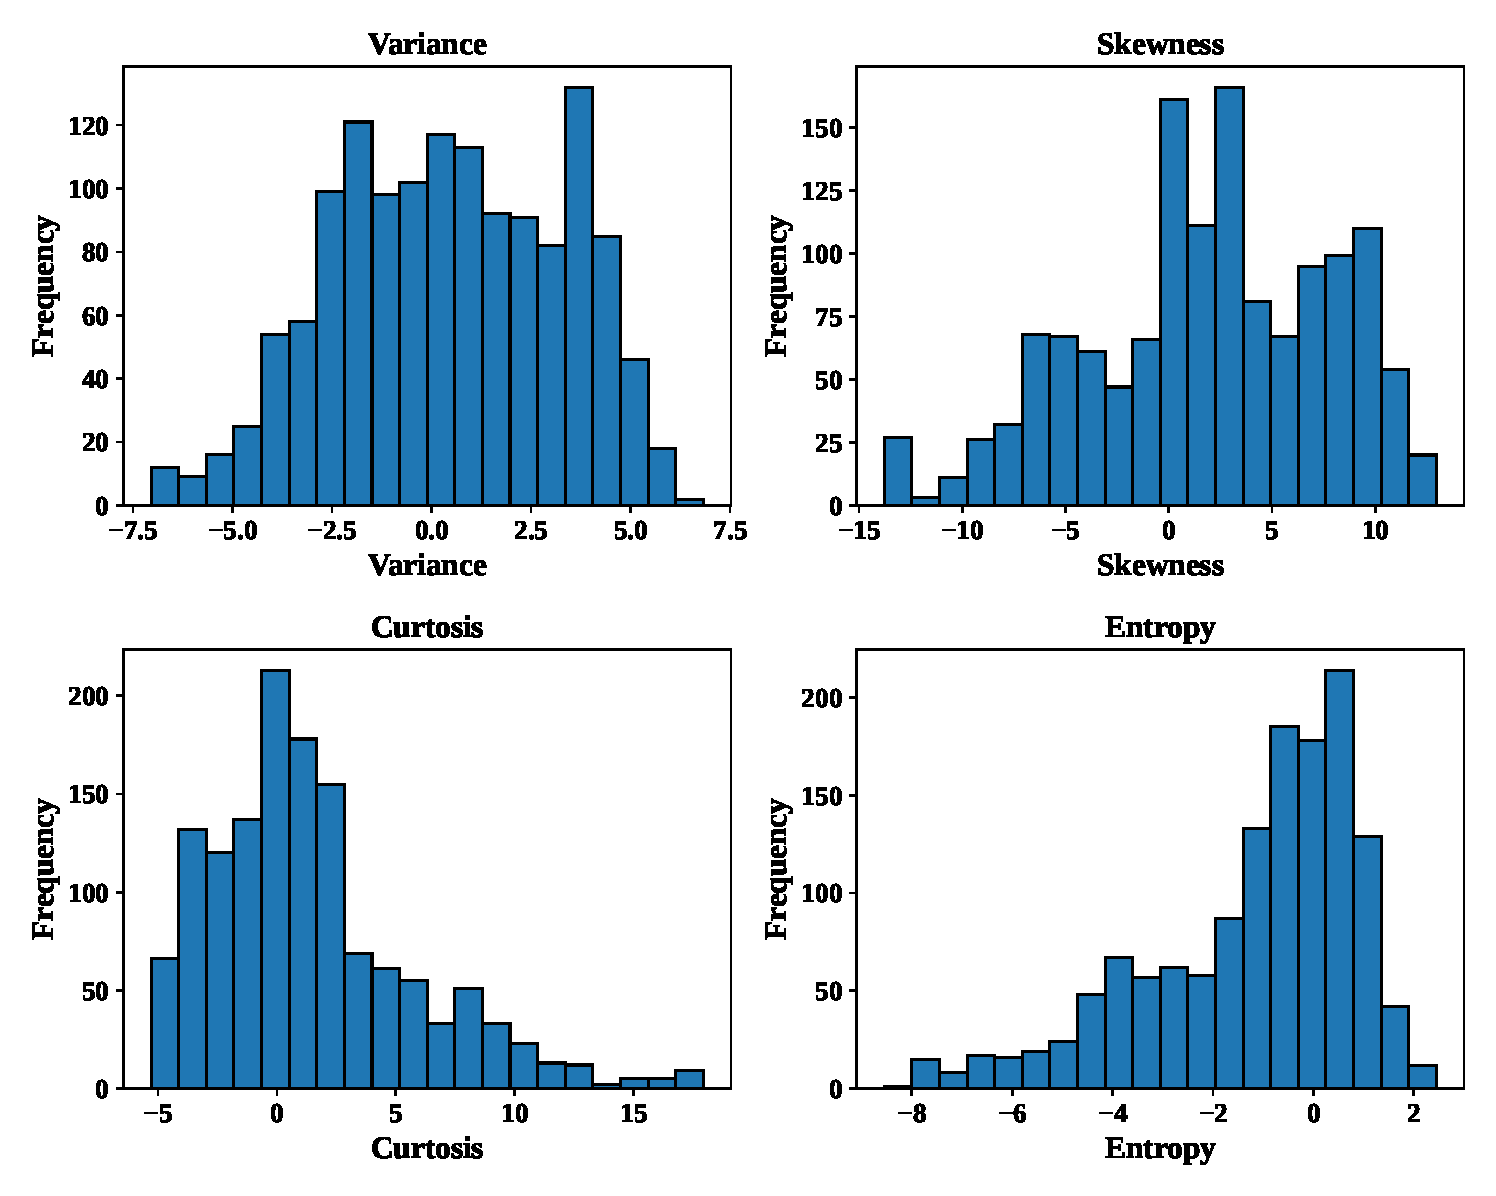
\includegraphics[width=\textwidth]{Histogram.eps}
\caption{Histograms of Dataset Features}
\end{figure}

\textbf{Interpretation:}

The Variance feature is distributed on negative and positive values. Skewness has multiple peaks showing different groups of data. Curtosis is positively skewed with long right tail, Entropy is negatively skewed with longer left tail. The different distributions and ranges imply that the features need to be normalised before training the perceptron.

%----------------------------------------------------------

\subsection{Correlation Heatmap}

\begin{figure}[H]
\centering
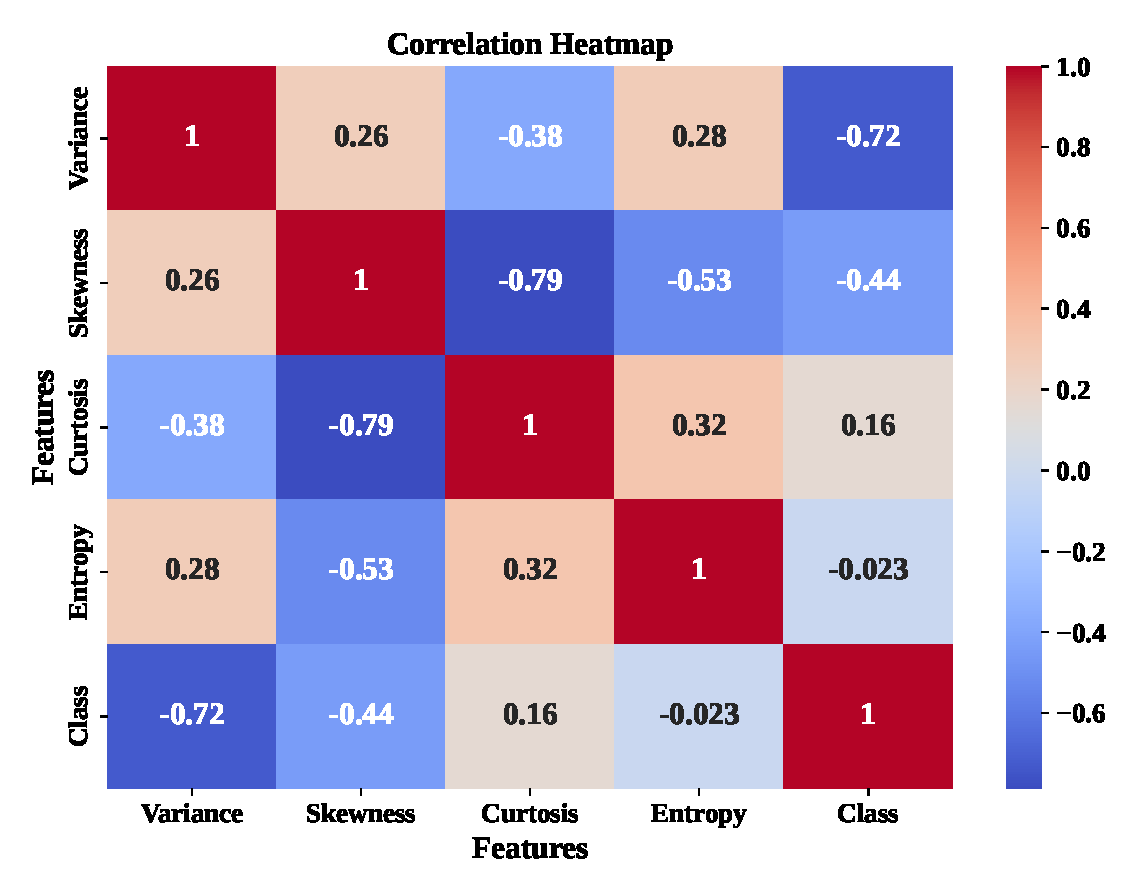
\includegraphics[width=\textwidth]{Correlation_Heatmap.eps}
\caption{Correlation Heatmap}
\end{figure}

\textbf{Interpretation:}

The heatmap shows a strong negative correlation of Variance and Class (-0.72), suggesting that Variance is an important feature for classification. Skewness and Curtosis are also highly negatively correlated (-0.79) and Entropy is very weakly correlated with the target class.

%----------------------------------------------------------

\subsection{Scatter Plot}

\begin{figure}[H]
\centering
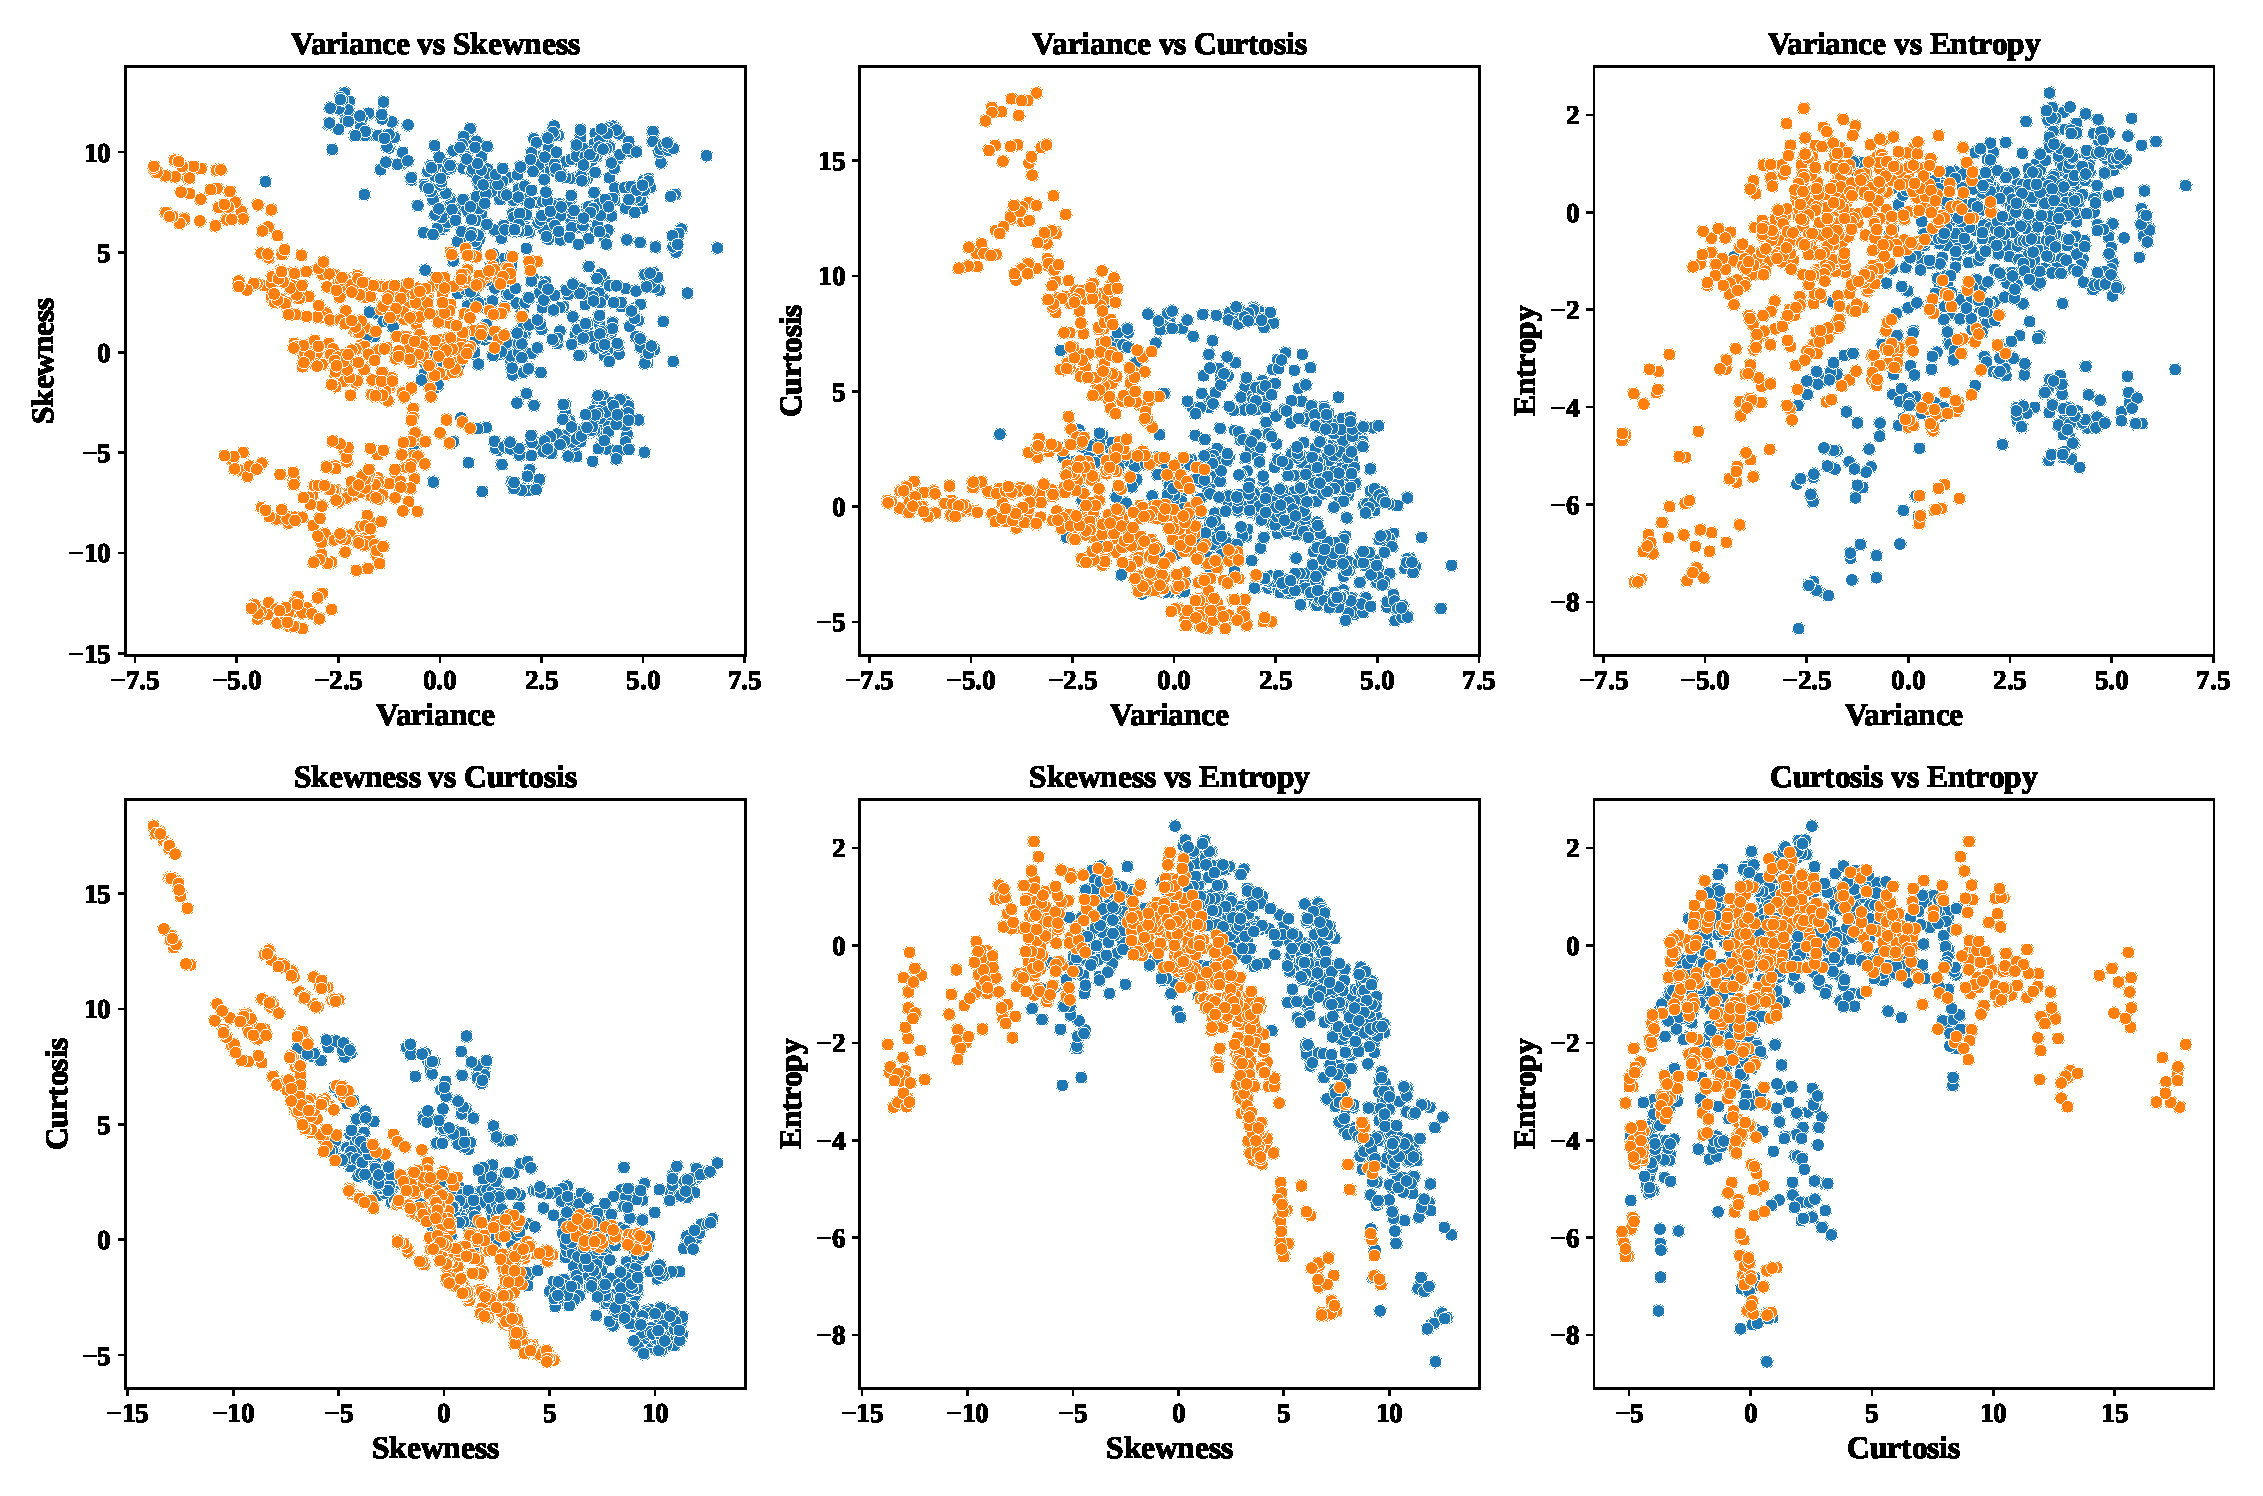
\includegraphics[width=\textwidth]{Scatter_Plot.eps}
\caption{Scatter Plot of Feature Combinations}
\end{figure}

\textbf{Interpretation:}

Variance combinations of features show the clearest class separation, but Curtosis vs Entropy has relatively more overlap. The dataset seems to be quite linearly separable.

%----------------------------------------------------------

\subsection{Boxplots}

\begin{figure}[H]
\centering
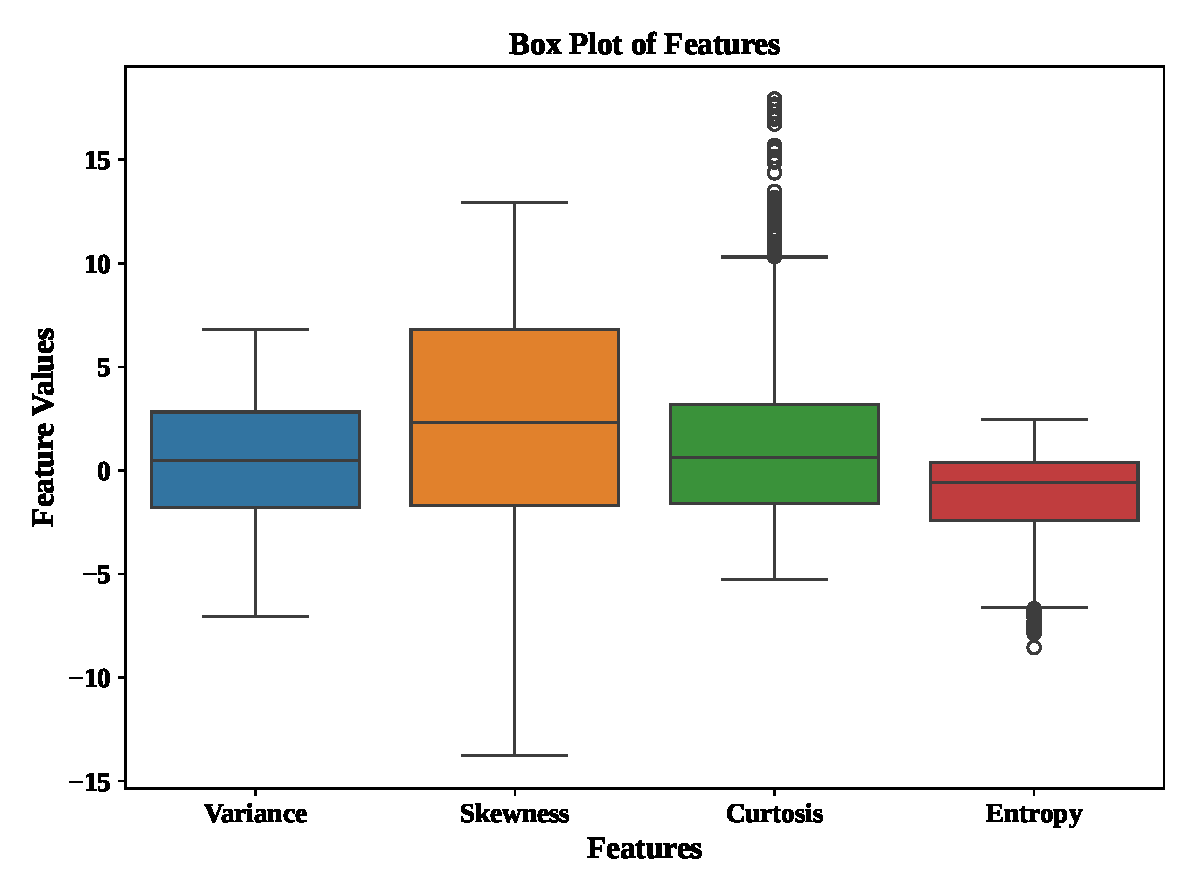
\includegraphics[width=\textwidth]{Box_Plot.eps}
\caption{Box Plot of Dataset Features}
\end{figure}

\textbf{Interpretation:}

Box plots indicate the difference in the range and spread of features. The maximum spread is observed in the case of skewness, and there are some outliers present in the Curtosis and Entropy features.

%----------------------------------------------------------

\subsection{Confusion Matrix}

\begin{figure}[H]
\centering
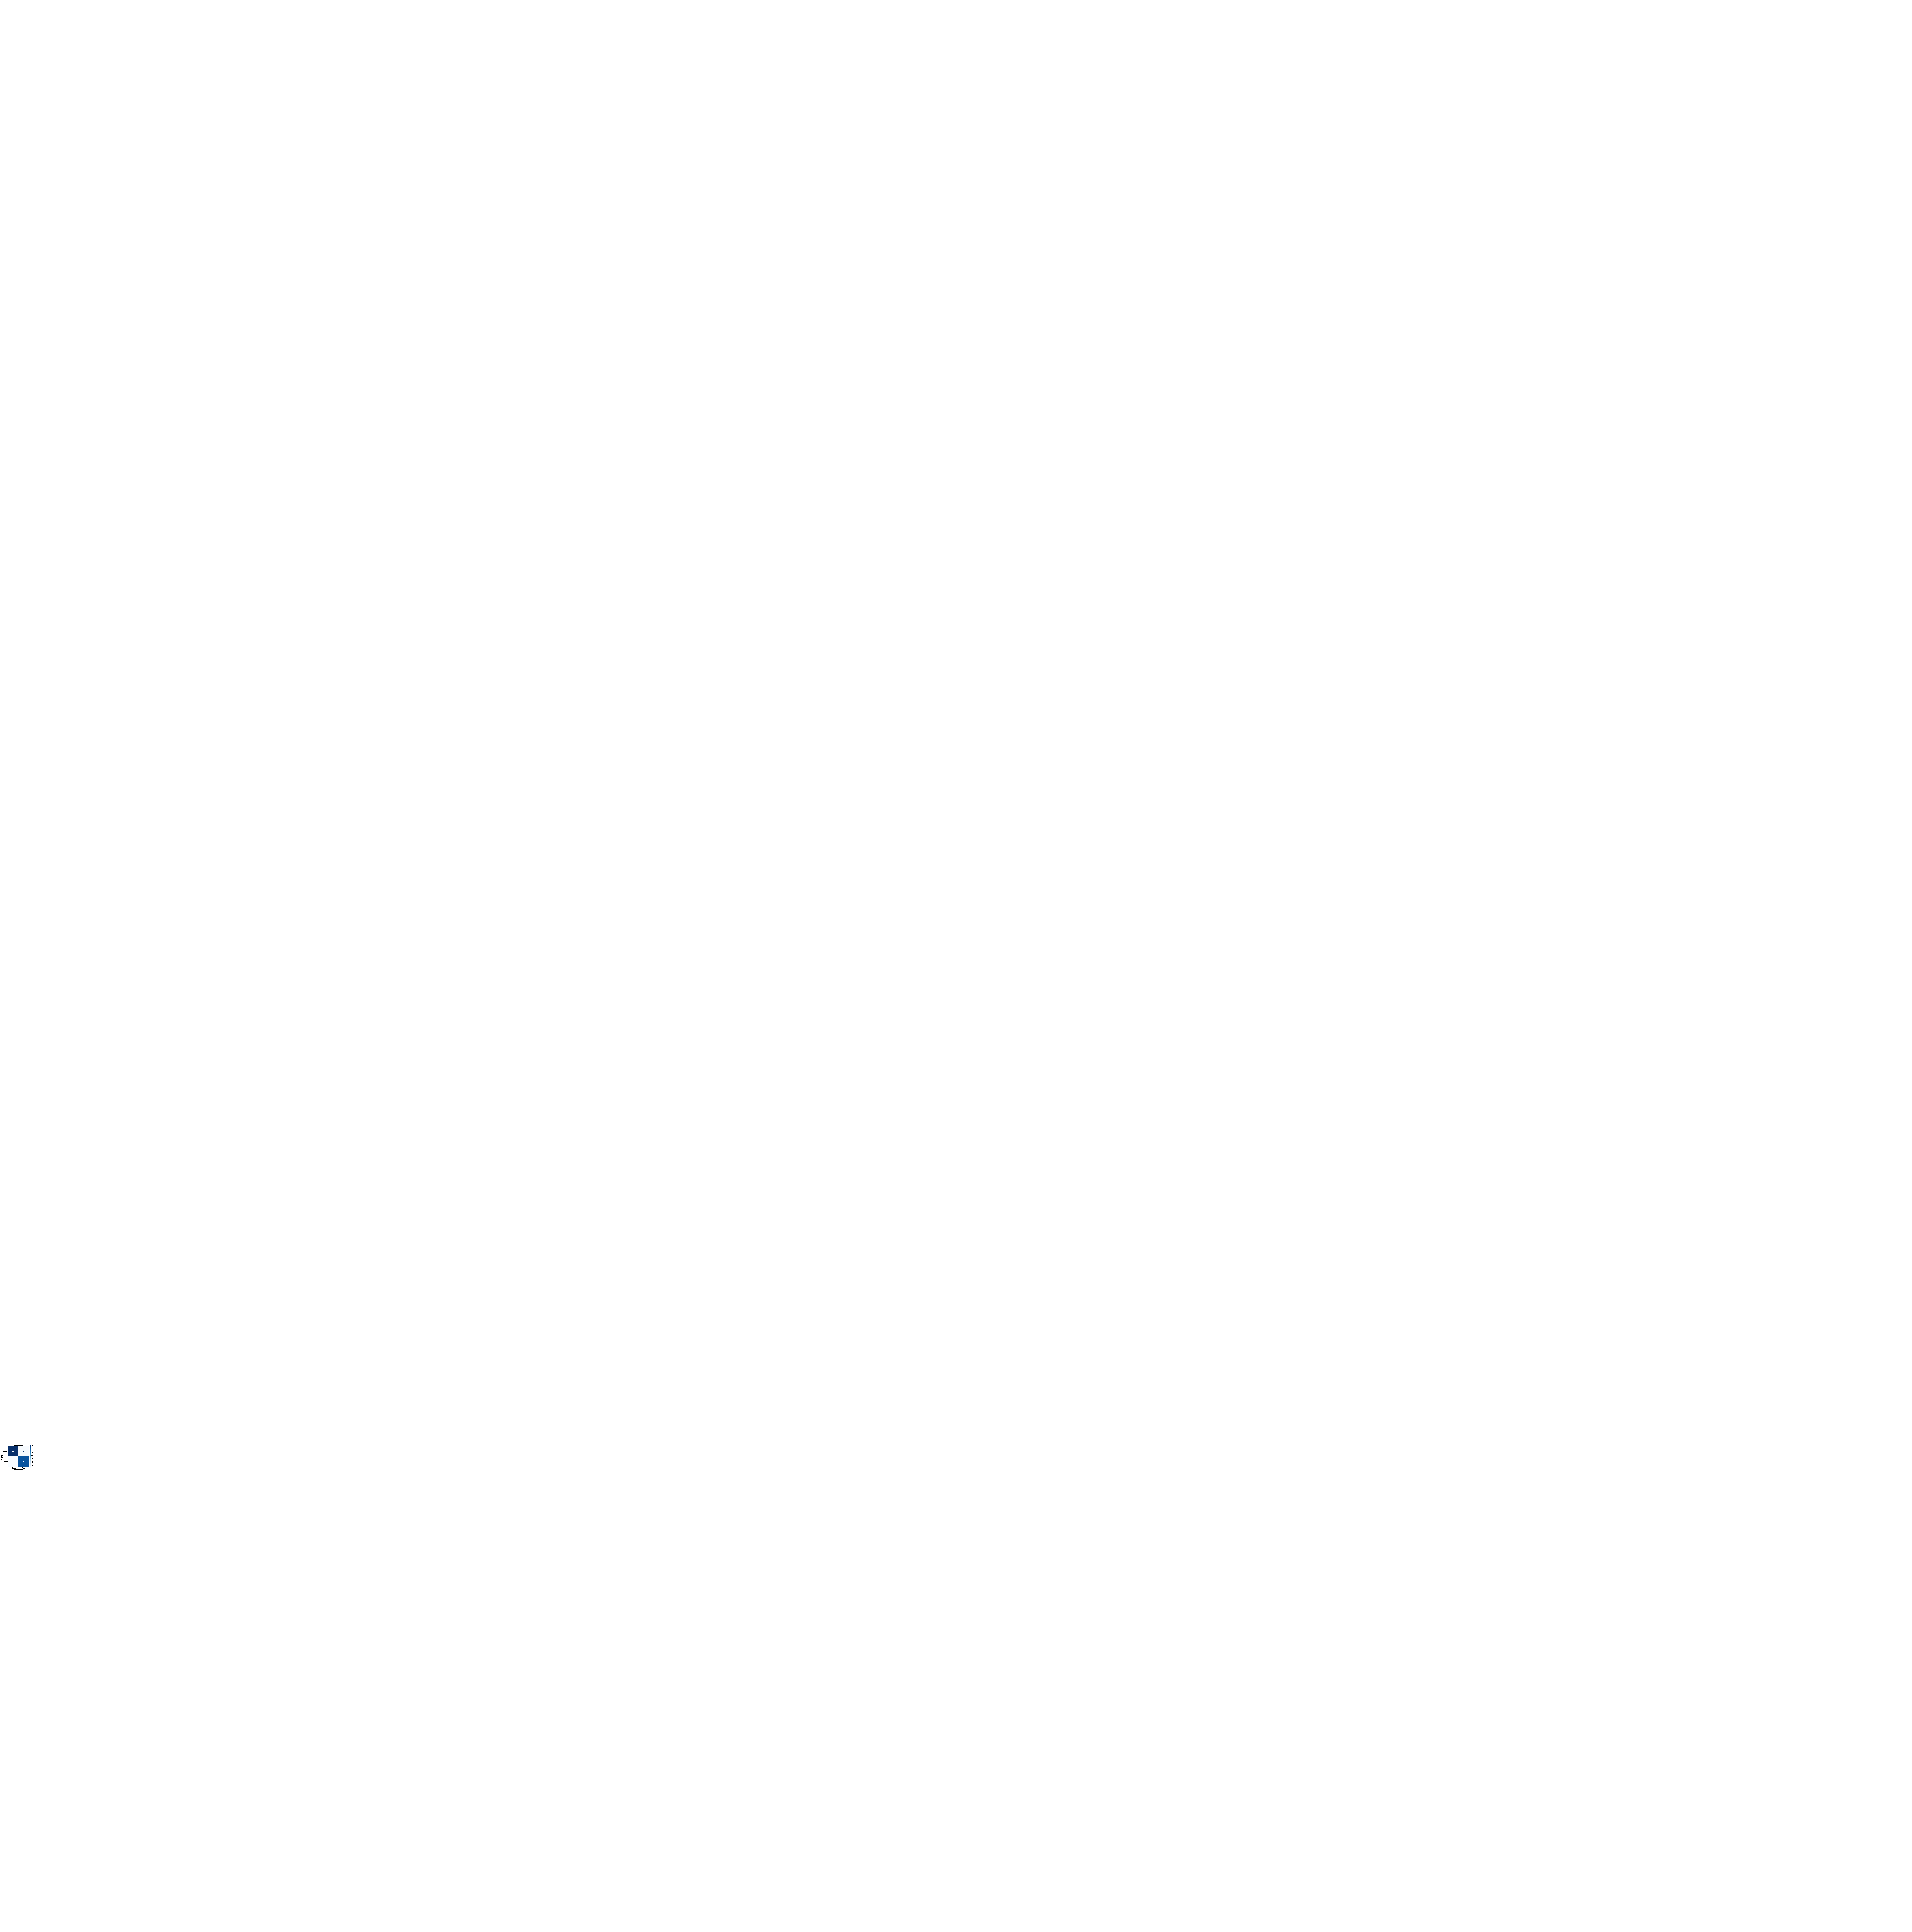
\includegraphics[width=0.75\textwidth]{Confusion_Matrix.eps}
\caption{Confusion Matrix}
\end{figure}

\textbf{Interpretation:}

Confusion matrix indicate that the perceptron was able to correctly classify 145 (TN) authentic banknotes as well as 125 (TP) forged banknotes. The classifier only made 5 errors out of the total 275 banknotes (3 (FP) authentic identified as forged and 2 (FN) forged as authentic).

%----------------------------------------------------------
\subsection{Training Error vs Epoch}

\begin{figure}[H]
\centering
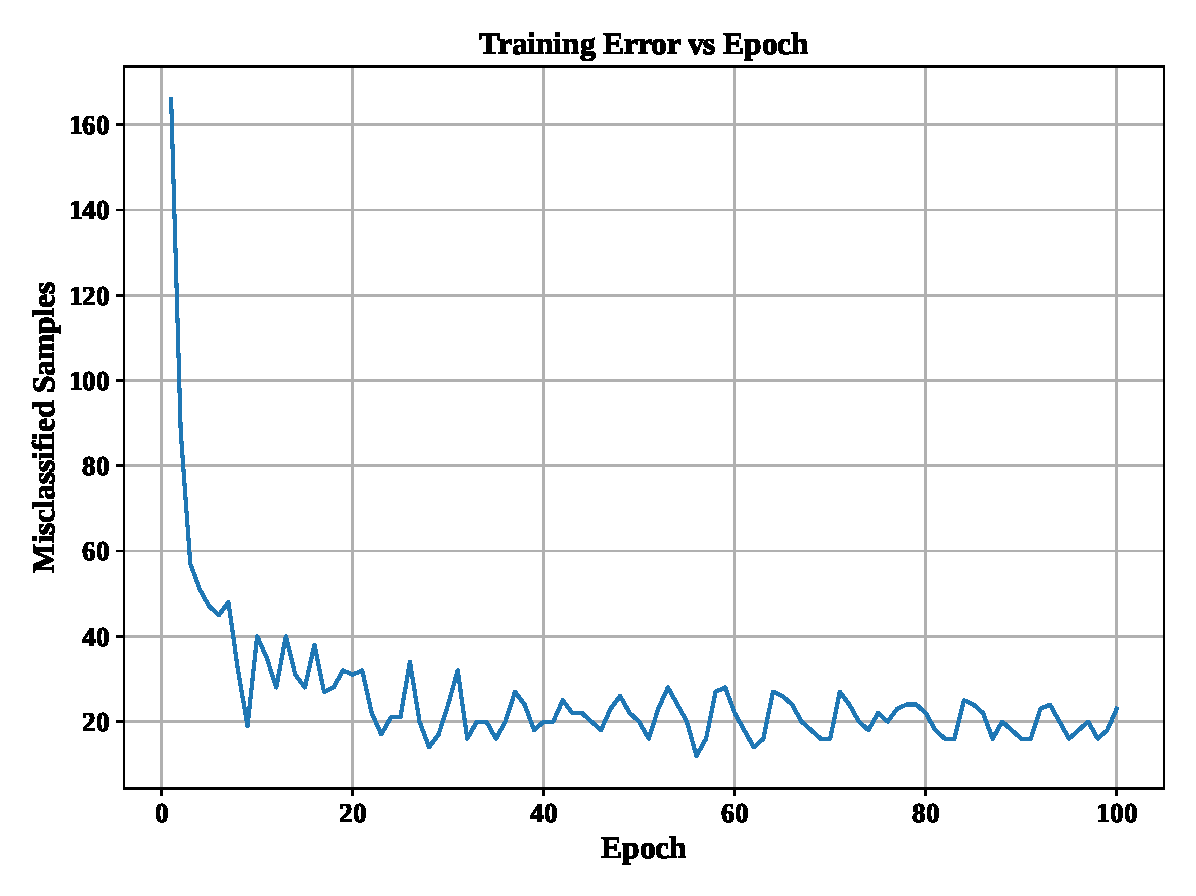
\includegraphics[width=0.9\textwidth]{Training_Error_vs_Epoch.eps}
\caption{Training Error versus Epoch}
\end{figure}

\textbf{Interpretation:}

The value of the training error reduces very fast at the beginning because the perceptron manages to learn the decision boundary. Once the number of epochs reaches about 20, the error starts to oscillate between 15 and 30 samples and does not reduce further. Thus, we can say that the perceptron has not fully achieved convergence.

%----------------------------------------------------------

\subsection{Weight Evolution}

\begin{figure}[H]
\centering
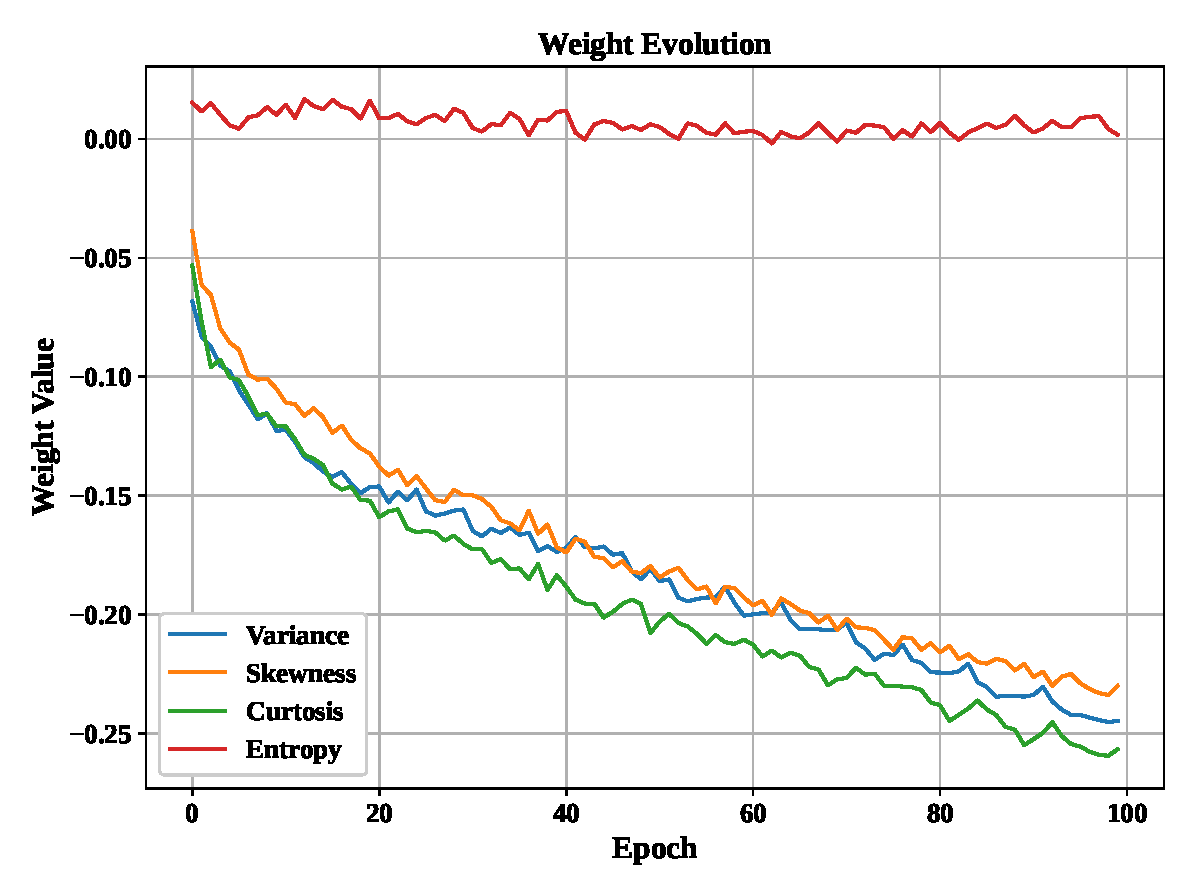
\includegraphics[width=0.9\textwidth]{Weight_Evolution.eps}
\caption{Evolution of Perceptron Weights}
\end{figure}

\textbf{Interpretation:}

There is considerable variation in the weights in the beginning stages of learning since the perceptron learns from the data provided to it during training. However, as training proceeds, the weights become stable with minor variations, suggesting that the model has learned a stable set of parameters.

%----------------------------------------------------------

\subsection{Bias Evolution}

\begin{figure}[H]
\centering
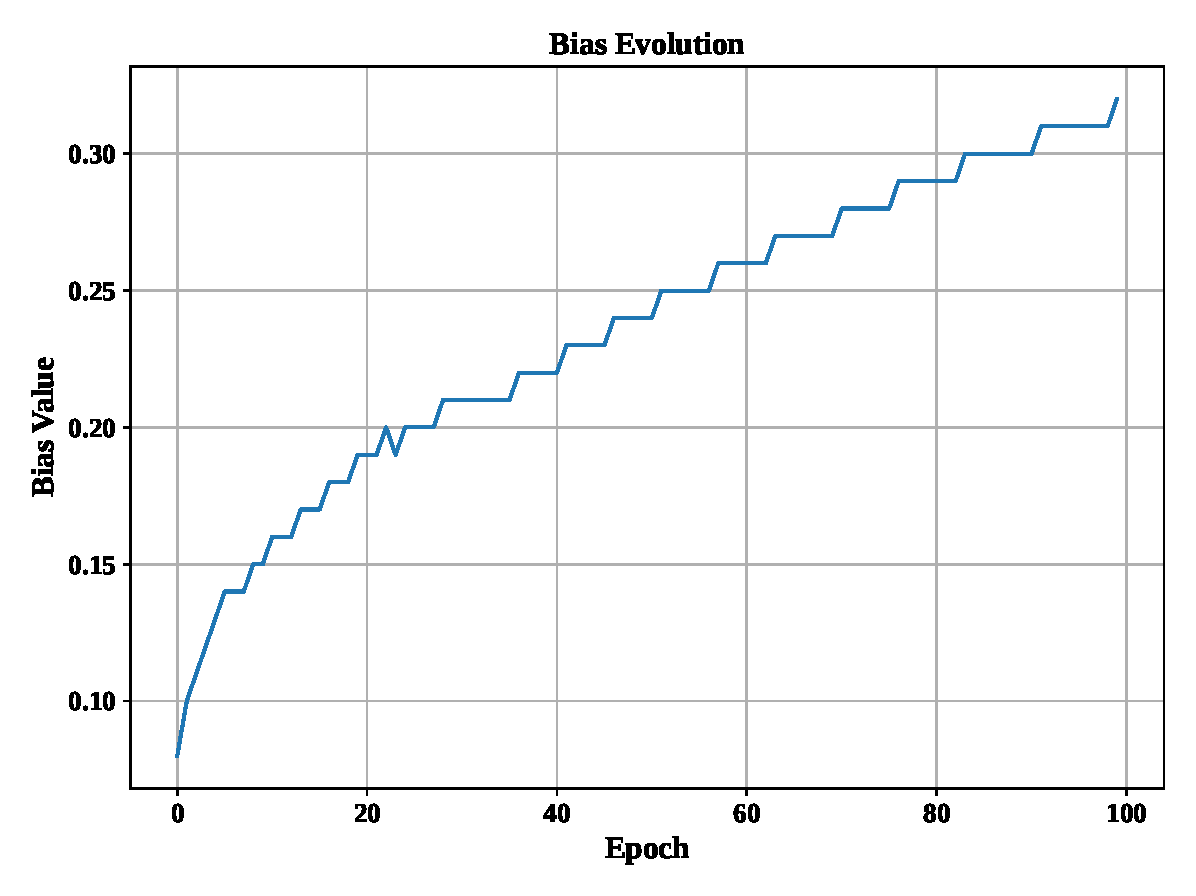
\includegraphics[width=0.9\textwidth]{Bias_Evolution.eps}
\caption{Evolution of Bias}
\end{figure}

\textbf{Interpretation:}

The increase is very fast in the early epochs, and then it becomes slower as time goes by. The stepping pattern shows that the bias only changes when there are misclassified samples, and it finally converges to 0.32, showing that the model has already learned a proper threshold for classification.

%----------------------------------------------------------

\subsection{Learning Rate Comparison}

\begin{figure}[H]
\centering
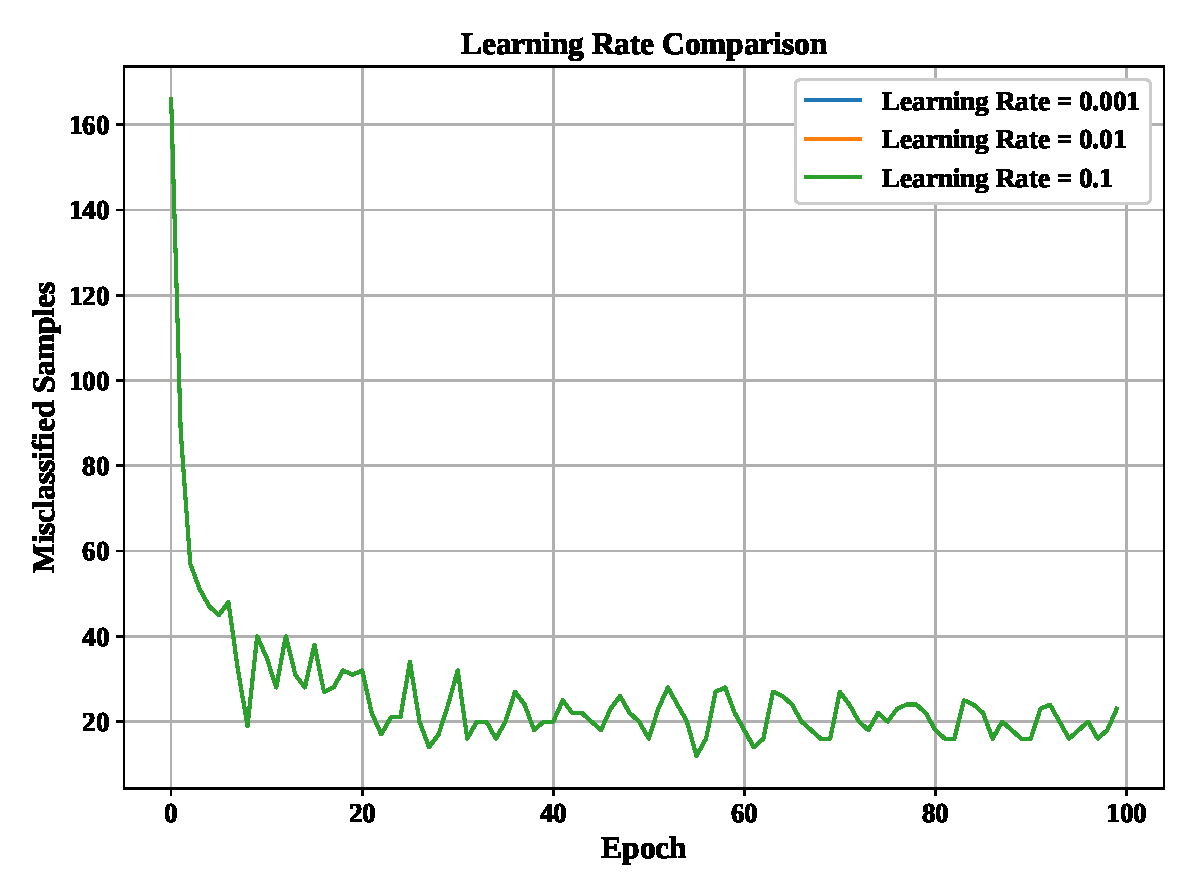
\includegraphics[width=0.9\textwidth]{Learning_Rate_Comparison.eps}
\caption{Comparison of Different Learning Rates}
\end{figure}

\textbf{Interpretation:}

The same curve is observed for all learning rates (0.001, 0.01, and 0.1) since perceptron weights are updated only when a sample is misclassified. As the data is almost linearly separable and has been scaled using MinMaxScaler, the same samples are misclassified every epoch. The only thing affected by learning rates is the magnitude of the change in the weights.

%----------------------------------------------------------

\section*{8. Performance Tables}

\textbf{Training Summary}

\begin{tabular}{|p{6cm}|p{7cm}|}
\hline
Dataset Size & 1372 Samples \\
\hline
Train/Test Split & 1097 Samples (80\%) and 275 Samples (20\%) \\
\hline
Learning Rate & 0.01 \\
\hline
Epochs & 100 \\
\hline
Final Weights & -0.2447762, -0.23011114, -0.25674323, 0.00175867 \\
\hline
Final Bias & 0.3200 \\
\hline
Accuracy & 0.9818 \\
\hline
Precision & 0.9766 \\
\hline
Recall & 0.9843 \\
\hline
F1-score & 0.9804 \\
\hline
\end{tabular}

\vspace{3mm}

\textbf{Epoch-wise Learning}

\begin{tabular}{|c|c|c|c|c|}
\hline
Epoch & Errors & Weight 1 & Weight 2 & Bias\\
\hline
1 & 166 & -0.06827408 & -0.03866853 & 0.08 \\
\hline
2 & 88 & -0.0831161 & -0.06146315 & 0.0999 \\
\hline
3 & 57 & -0.08731574 & -0.0656554 & 0.1099 \\
\hline
4 & 51 & -0.09538568 & -0.07974311 & 0.1199 \\
\hline
5 & 47 & -0.09778344 & -0.0856403 & 0.1299 \\
\hline
$\vdots$ & $\vdots$ & $\vdots$ & $\vdots$ & $\vdots$ \\
\hline
100 & 23 & -0.2447762 & -0.23011114 & 0.3200 \\
\hline
\end{tabular}

%----------------------------------------------------------

\section*{9. Discussion}

\begin{enumerate}[leftmargin=*]
\item \textbf{Compare the Step and Sigmoid activation functions. Discuss why the Step Activation Function is not used in modern deep learning models.}

Step Activation Function gives the output as either 0 or 1, while the Sigmoid Activation Function gives an output that varies continuously from 0 to 1. The Step function is never used in deep learning since it is not differentiable and hence cannot be used in backpropagation. This is the reason why Sigmoid and other activation functions are used.

\item \textbf{Compare the implementation with Scikit-learn's Perceptron.}

The perceptron that has been developed is an implementation of the basic perceptron learning rule, where weights and biases are adjusted manually. The Scikit-learn Perceptron, on the other hand, is highly optimized and incorporates functions like shuffling data, early stopping, and regularization.

\item \textbf{Repeat the experiment using learning rates 0.001, 0.01 and 0.1.}

In this case, the experiments were done using the learning rates of 0.001, 0.01 and 0.1. All three learning rates converged similarly and performed almost equally well. The learning rate impacted mainly the size of weight changes rather than affecting the accuracy of classification.

\item \textbf{Explain why a Single Layer Perceptron cannot solve the XOR problem.}

Single Layer Perceptron can classify only linearly separable data. As the XOR problem is not linearly separable, a single decision boundary cannot distinguish its classes. Hence, Multilayer Perceptron is needed for solving the XOR problem.

\item \textbf{Study the effect of feature normalization on model convergence.}

Feature scaling will ensure that all input features have a standard scale value, thereby avoiding the domination of any feature with higher value. In the current experiment, MinMax scaling will increase training stability and allow for faster convergence of the perceptron.
\end{enumerate}

%----------------------------------------------------------

\section*{10. Additional tasks}

\subsection{Perceptron learning algorithm for OR Gate}

\begin{figure}[H]
\centering
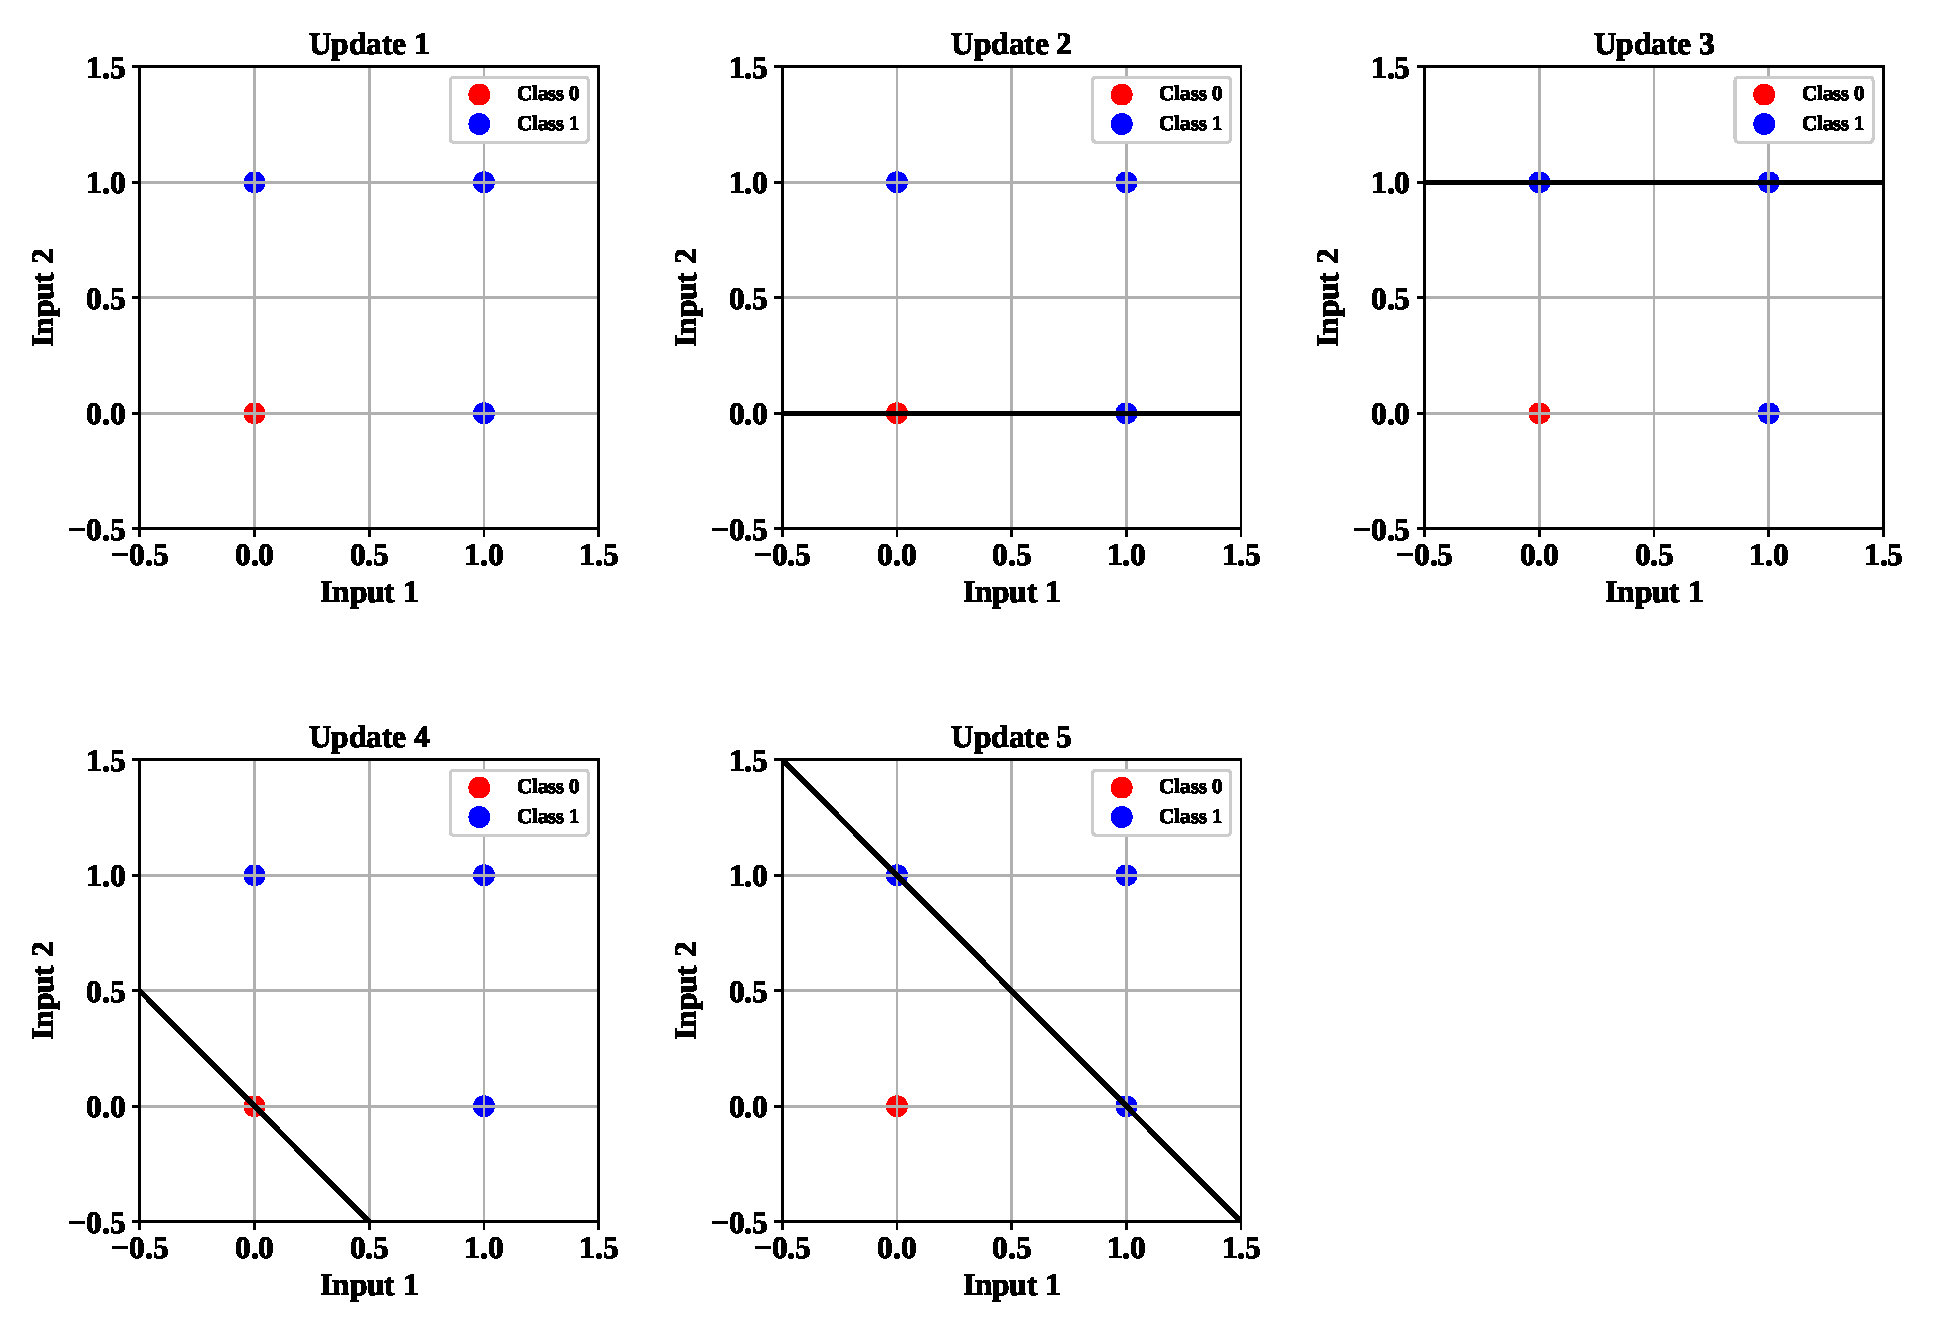
\includegraphics[width=\textwidth]{OR_Decision_Boundaries.eps}
\caption{OR Gate Decision Boundaries}
\end{figure}

\textbf{Interpretation:}

The decision boundary is changing after each weight update, and it gradually separates the OR gate inputs into correct classes and shows the perceptron learning process.
%----------------------------------------------------------

\subsection{Perceptron learning algorithm for AND Gate}

\begin{figure}[H]
\centering
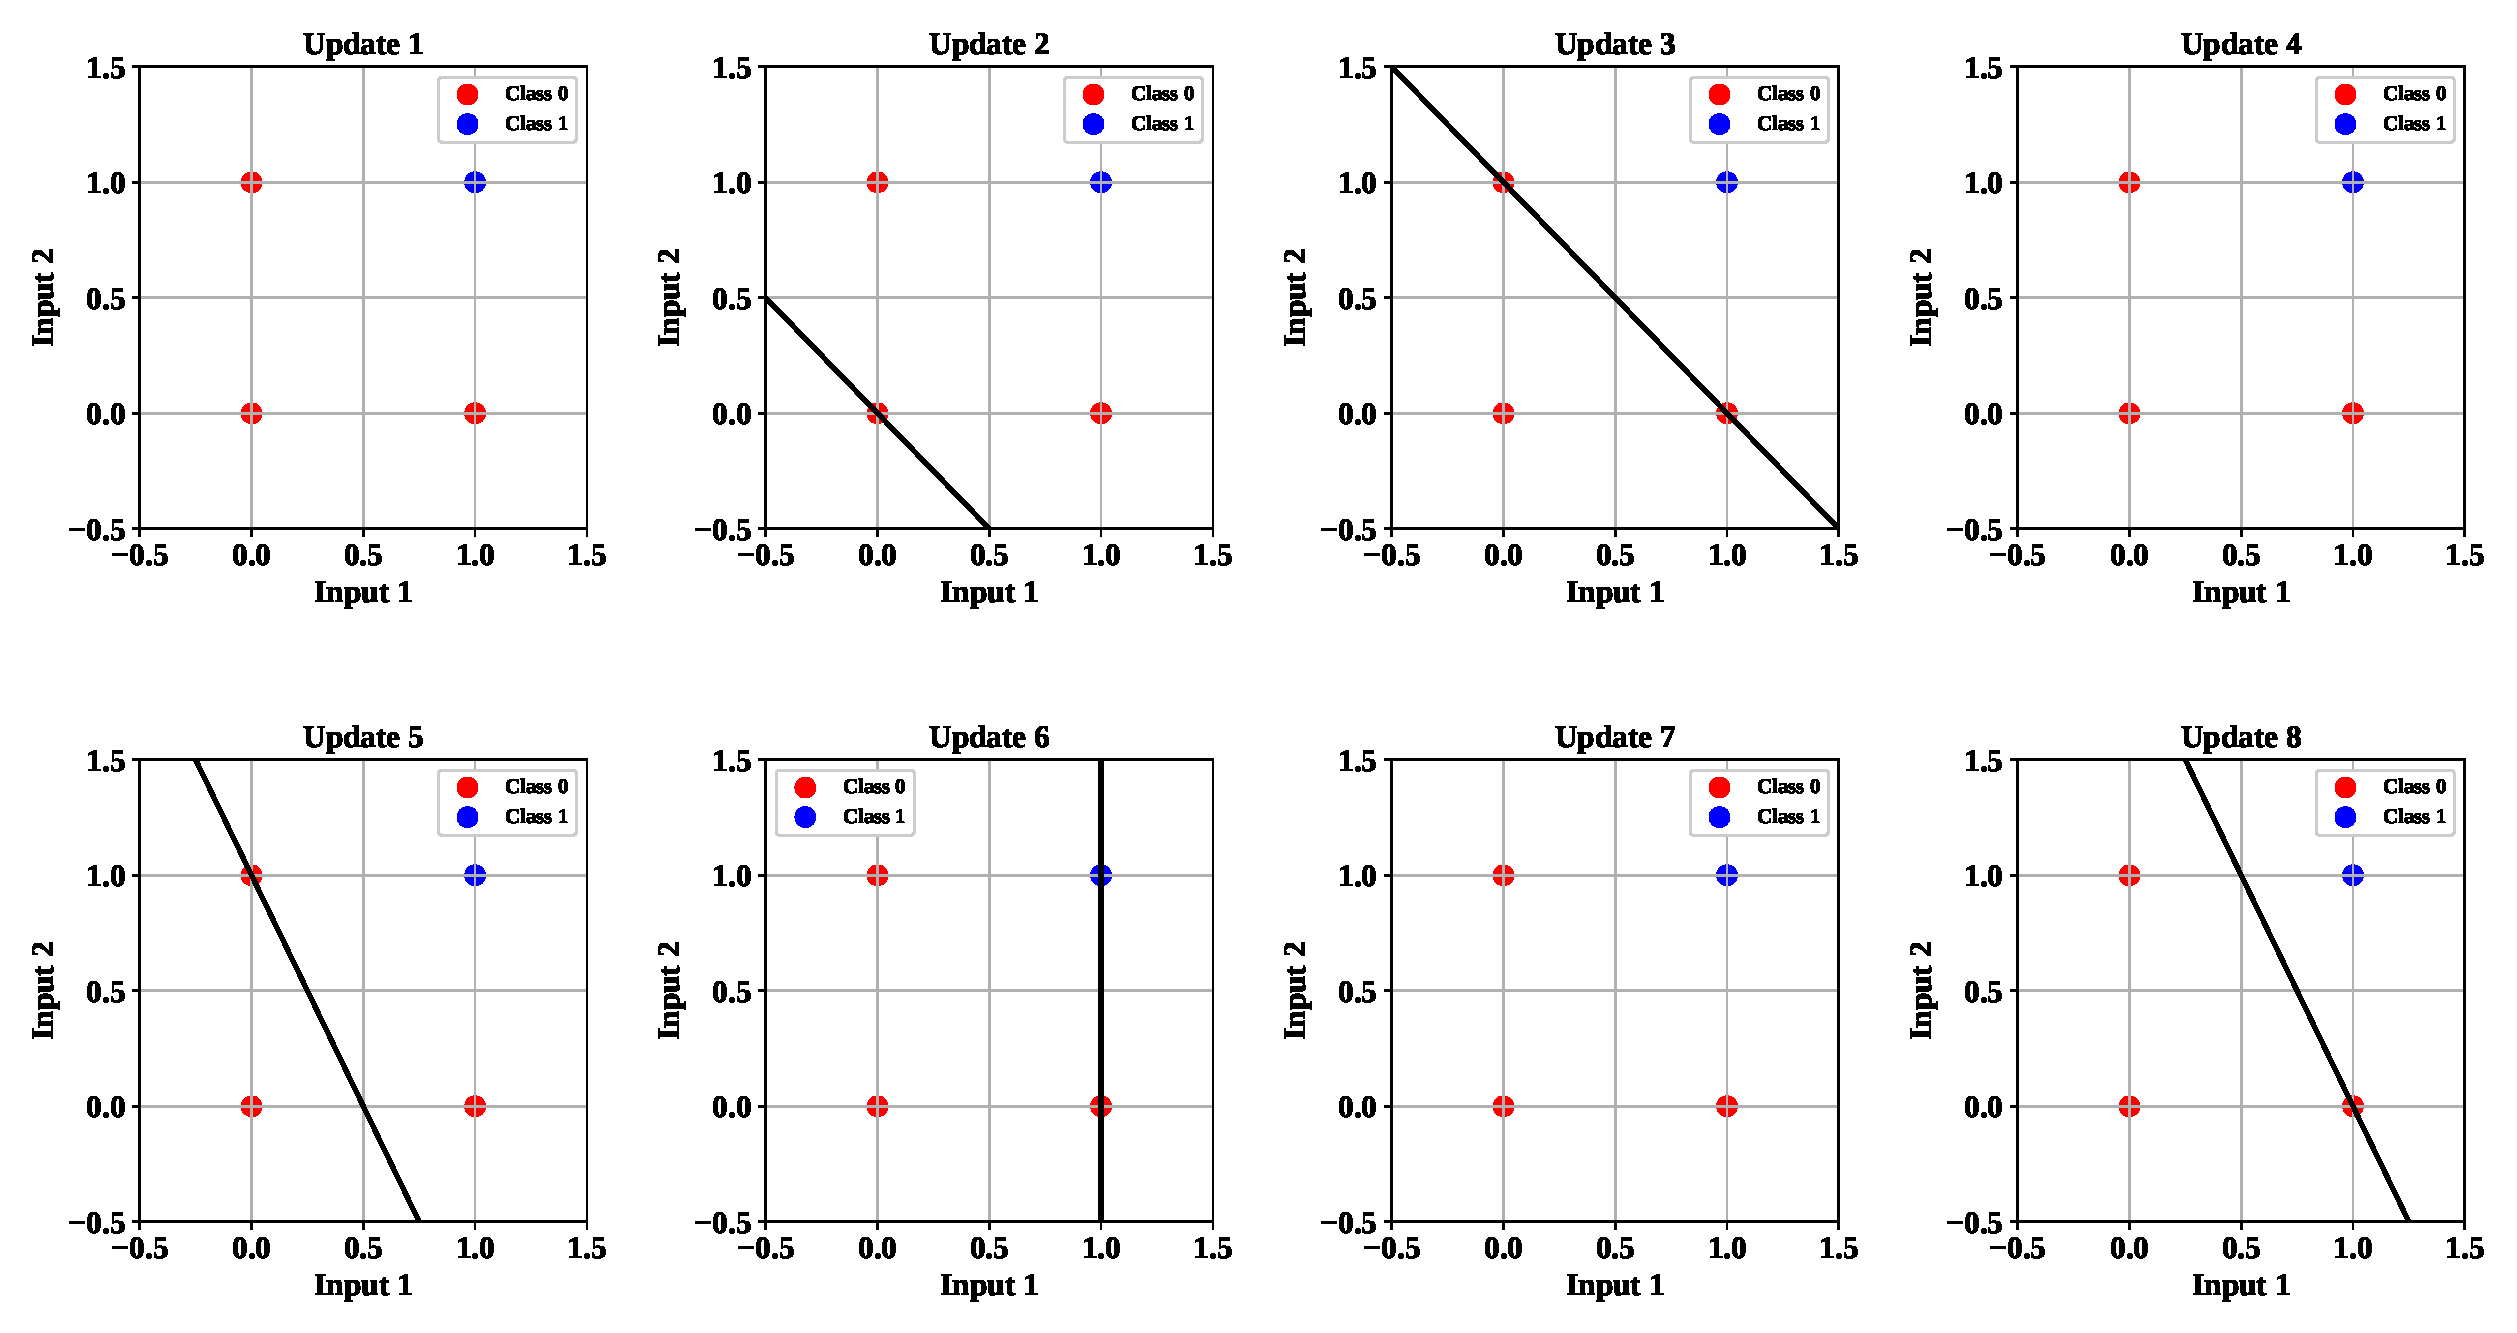
\includegraphics[width=\textwidth]{AND_Decision_Boundaries.eps}
\caption{AND Gate Decision Boundaries}
\end{figure}

\textbf{Interpretation:}

The decision boundary is changing after each weight update and gradually moving to separate the single positive class (1,1) from the rest negative samples, showing the perceptron learning process.
%----------------------------------------------------------

\subsection{Perceptron learning algorithm for NOT Gate}

\begin{figure}[H]
\centering
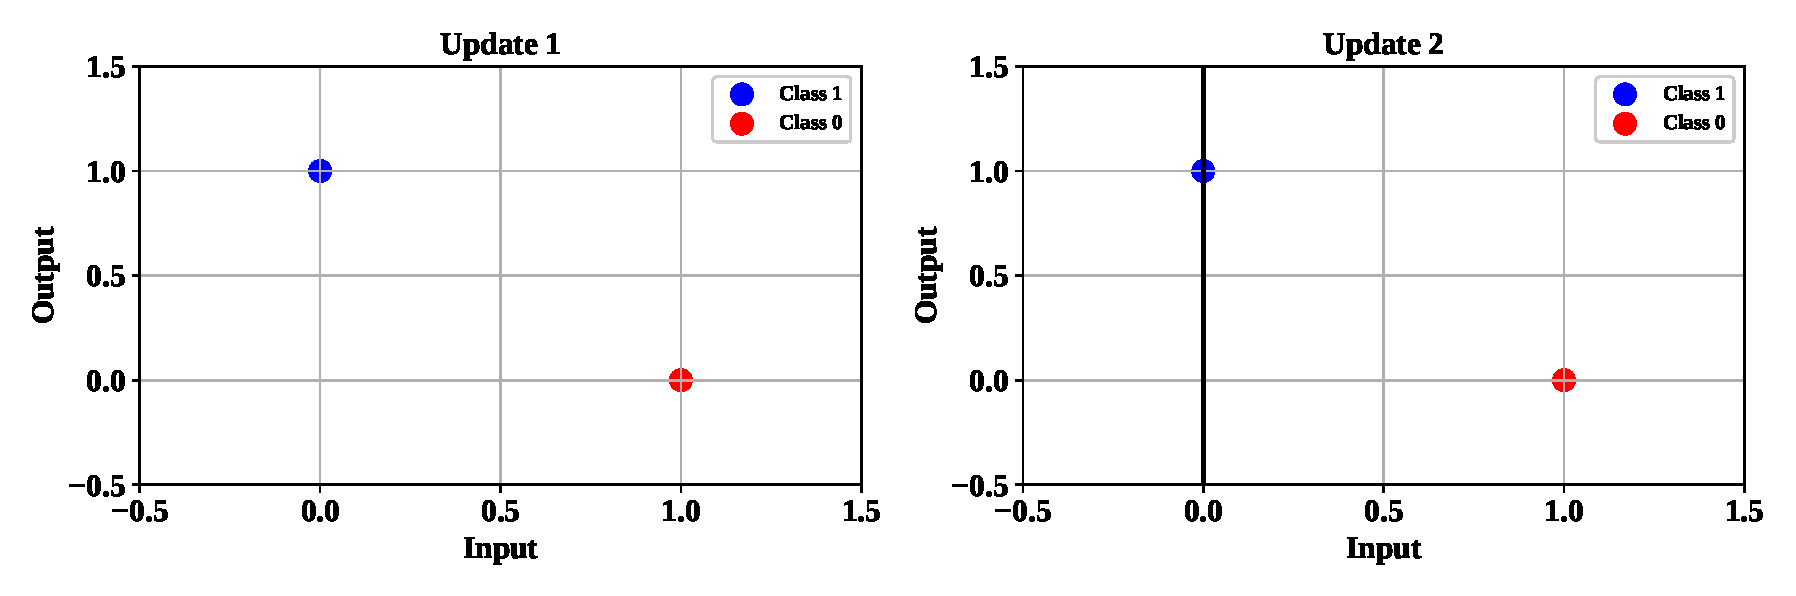
\includegraphics[width=\textwidth]{NOT_Decision_Boundaries.eps}
\caption{NOT Gate Decision Boundaries}
\end{figure}

\textbf{Interpretation:}

The perceptron learns the NOT gate in just 2 weight updates. This means that the data is linearly separable. After the second update the decision boundary quickly stabilises and both input samples are correctly classified with successful convergence.
%----------------------------------------------------------

\section*{11. Conclusion}

In the experiment, the Single Layer Perceptron was successfully developed for the purpose of classifying the Banknote Authentication dataset into two classes. For this, the dataset was normalized through MinMax technique while the perceptron learning algorithm and step activation function were used to train the classifier. As a result, the classifier performed extremely well on linearly separable data.

%----------------------------------------------------------

\section*{12. References}

\begin{enumerate}
\item F. Rosenblatt, ``The Perceptron,'' \emph{Psychological Review}, 1958.
\item I. Goodfellow, Y. Bengio and A. Courville, \emph{Deep Learning}, MIT Press, 2016.
\item C. M. Bishop, \emph{Pattern Recognition and Machine Learning}, Springer, 2006.
\item S. Haykin, \emph{Neural Networks and Learning Machines}, Pearson, 2009.
\item UCI Machine Learning Repository -- Banknote Authentication Dataset.
\item Scikit-learn Documentation: Perceptron.
\end{enumerate}

\end{document}